\cotefile{138}
\scanpage{46}
% archive foliation: 45
% lines 1-3
Posons pour abréger $X=C_2$, soit $D$ le diviseur de ramification sur $X$ (de degré 6) -- son corps de décomposition est $Q(i)$; \deleted{\unsure{posons} $X^*=X\setminus D$}\inserted{posons $X^*=X\setminus D$},
% line 4
\deleted{et soit $\widetilde X^*$ le rev. universel abélien de $X^*$}
% lines 5-7
Soit $X_\infty$ le \inserted{pro-}\unsure{rev\textsuperscript{t}} \deleted{abélien}\inserted{principal} de $X$ défini par la famille des $\unsure{C_n}$ ($n$ pairs), il a comme \unsure{groupe} $(\Pi_\infty)\deleted{_{\unsure{X_2|X_*}}}$

\scanpage{47}
% archive foliation: 46
% lines 1-5, upper-left diagram
\figure{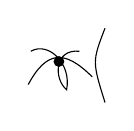
\begin{tikzpicture}[scale=.65]
\draw (-.55,.2) .. controls (-.2,.4) and (.25,-.05) .. (.15,-.55) .. controls (-.1,-.35) and (-.1,.25) .. (.4,.2);
\draw (-.6,-.45) .. controls (-.25,.2) and (.1,.25) .. (.65,-.3);
\fill (0,0) circle (3pt);
\draw (.9,.65) .. controls (.65,0) .. (.9,-.8);
\end{tikzpicture}}
\diagram{\begin{tikzcd}[row sep=large,column sep=large]
X_n=\unsure{\operatorname{Sp\hat ec}} k[x_n] \arrow[d] & \deleted{\unsure{x_n}}x_n^n=x_1 \\
X_1=\unsure{\operatorname{Sp\hat ec}} k[x_1=z] \arrow[d] & \left[\begin{array}{ccc}n&\vdots&n\end{array}\right] \\
X_0=\unsure{\operatorname{Sp\hat ec}} k[u] & \left[\begin{array}{ccc}2&2&\vdots\end{array}\right]
\end{tikzcd}}
\figure{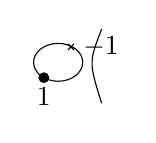
\begin{tikzpicture}[scale=.65]
\draw (0,0) ellipse (.48 and .37);\fill (-.28,-.3) circle (3pt);
\node[below] at (-.28,-.3) {$1$};\draw (.25,.3) ++(-.06,-.06)--++(.12,.12);\draw (.25,.3) ++(-.06,.06)--++(.12,-.12);\node[right] at (.3,.3) {$-1$};
\draw (.85,.65) .. controls (.6,0) .. (.85,-.8);
\end{tikzpicture}}
\[
u=\frac12-\frac14(z+z^{-1})
\]
% lines 2-4, upper-right
ramification au-dessus des \unsure{p\textsuperscript{ts}} $0,\infty$ (où la ramification est $n$)

\unsure{p\textsuperscript{ts}} de ramification en haut : $0,\infty$
% lines 5-9, upper-right
ramification au dessus de
\[
\begin{array}{ll}
0 & \deleted{\unsure{pas ramifié}\ (\unsure{p\textsuperscript{ts} au dessus}}\inserted{(z=1\ \text{ramification }2)}\\
1 & (z=-1,\ \text{ramification }2)\\
 & \deleted{\unsure{idem}}\\
\infty & (0\text{ et }\infty\ \text{ramification }1)
\end{array}
\]
% line 6, left
\[
D_\infty=(Z_{/2})\mathbin{\underset{\unsure{1/2}}{\cdot}}\mu_\infty
\]
% lines 10-14, middle diagrams
\diagram{\begin{tikzcd}[row sep=large,column sep=small]
0\ (n)\arrow[d]& &\infty\ \unsure{(n)}\arrow[d]&1\ (1)\arrow[d,"{n\ \text{fois}}"{description,draw,ellipse}]&\deleted{\unsure{-1|\infty}\ (1)}\arrow[d,draw=none,"{\deleted{\downarrow}}"{description}]&\text{$n$ pair}\\
0\ (1)\arrow[dr]&&\infty\ (1)\arrow[dl,dash]&1\ (2)\arrow[d]&-1\ \deleted{\unsure{0\ (2)}}\ (2)\arrow[d]&\\
&\infty&&0&1&
\end{tikzcd}}
\figure{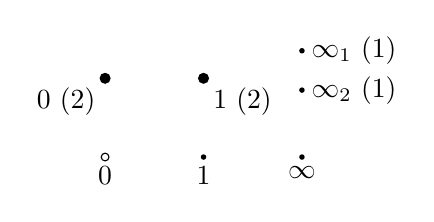
\begin{tikzpicture}[x=1.25cm,y=1cm]
\fill (0,0) circle (2pt);\node[below left] at (0,0) {$0\ (2)$};
\fill (1,0) circle (2pt);\node[below right] at (1,0) {$1\ (2)$};
\fill (2,.35) circle (1pt);\node[right] at (2,.35) {$\infty_1\ (1)$};
\fill (2,-.15) circle (1pt);\node[right] at (2,-.15) {$\infty_2\ (1)$};
\draw (0,-1) circle (1.4pt);\node[below] at (0,-1) {$0$};
\fill (1,-1) circle (1pt);\node[below] at (1,-1) {$1$};
\fill (2,-1) circle (1pt);\node[below] at (2,-1) {$\infty$};
\end{tikzpicture}}
% lines 15-17, lower graph
\figure{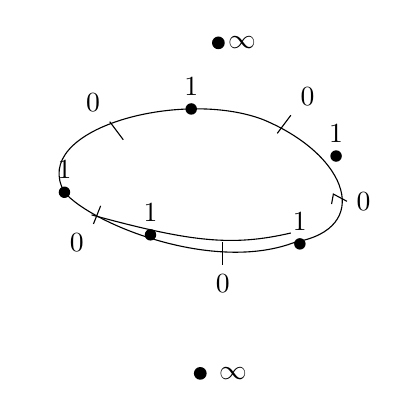
\begin{tikzpicture}[scale=1.15]
\fill (.2,1.65) circle (2pt);\node[right] at (.2,1.65) {$\infty$};
\draw (-1.5,0) .. controls (-1.9,.7) and (-.2,1.15) .. (.7,.8);
\draw (.7,.8) .. controls (1.65,.4) and (1.9,-.4) .. (1.05,-.55) .. controls (.15,-.9) and (-1.2,-.35) .. (-1.5,0);
\draw (-1.2,-.25) .. controls (-.1,-.55) and (.35,-.6) .. (1,-.45);
\foreach \x/\y/\lab in {-1.5/0/1,-.1/.92/1,1.5/.4/1,1.1/-.57/1,-.55/-.47/1}{\fill (\x,\y) circle (1.8pt);\node[above] at (\x,\y+.04) {$\lab$};}
\draw (-1,.78)--(-.85,.58);\node[above left] at (-1,.78) {$0$};
\draw (.85,.65)--(1,.85);\node[above right] at (1,.85) {$0$};
\draw (1.62,-.1)--(1.47,-.02)--(1.45,-.13);\node[right] at (1.62,-.1) {$0$};
\draw (.25,-.55)--(.25,-.8);\node[below] at (.25,-.8) {$0$};
\draw (-1.1,-.15)--(-1.18,-.35);\node[below left] at (-1.18,-.35) {$0$};
\fill (0,-2) circle (2pt);\node[right] at (.1,-2) {$\infty$};
\end{tikzpicture}}
% lines 18-19, inverted printed label
\begin{tabular}{l}
MR LE PROFESSEUR GROTHENDIECK A.\\
MATHEMATIQUES\qquad 5
\end{tabular}

\scanpage{48}
% archive foliation: 47
% The typed sheet is upside down in the supplied scan; order below follows the upright sheet.
% lines 1-3
ACADEMIE DE MONTPELLIER

\texttt{----------}

JC/JV

LE RECTEUR DE L'ACADEMIE DE MONTPELLIER

Chancelier des Universités
% lines 4-6
VU\qquad la loi N° 68-978 du 12 novembre 1968 d'orientation de l'enseignement supérieur et notamment son article 18
% lines 7-10
VU\qquad la démission présentée par M. le Profes-\\
seur Jacques ROUZAUD, administrateur provisoire de l'Université de MONTPELLIER II
% lines 11-12
\begin{center}
A R R E T E\\
\texttt{-----------}
\end{center}
% lines 13-18
\uline{Article premier}.

La démission de M. le Professeur Jacques ROUZAUD de ses fonctions d'administrateur provisoire de l'Université de Montpellier II est acceptée à compter du 26 juin 1978 et l'arrêté rectoral du 15 décembre 1977 est abrogé à la même date.
% lines 19-24
\uline{Article deux.}

Monsieur Yvan MEYERHOEFFER, Conseiller du Tribunal Administratif de Montpellier, est chargé des fonctions d'administrateur provisoire de l'Université de Montpellier II à compter du 27 juin 1978 et jusqu'à la date d'installation d'un président élu.
% lines 25-26
Fait à Montpellier, le 27 Juin 1978

LE RECTEUR,
% line 27, signature
\figure{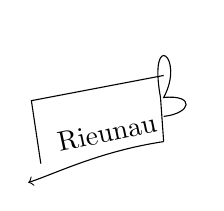
\begin{tikzpicture}[scale=.8]
\node[rotate=12] at (0,0) {\unsure{Rieunau}};
\draw (.9,.9)--(-1.2,.5)--(-1.05,-.5);
\draw (.9,-.15)--(.85,.55) .. controls (.65,1.65) and (1.25,1.2) .. (.9,.55) .. controls (1.4,.6) and (1.35,.3) .. (.9,.25);
\draw[->] (.9,-.15) .. controls (-.1,-.3) and (-.8,-.65) .. (-1.25,-.8);
\end{tikzpicture}}
% lines 28-30, lower left
\uline{Diffusion} : liste D

n° 4027

MONTPELLIER, le 27 Juin 1978

\scanpage{49}
% archive foliation: 48
% lines 1-3
\[
\begin{aligned}
z'&=z^3\\
y'&=y(y^2-3x^2)\\
x'&=-x(x^2-3y^2)
\end{aligned}
\]
% lines 4-6
\[
\begin{aligned}
&z^6+y^2(y^4+9x^4-6x^2y^2)+x^2(x^4+9y^4-6x^2y^2)\\
&=x^6+y^6+z^6+\unsure{3|9}x^2y^2(x^2+y^2)=\deleted{(x^2+y^2+z^2)^3}\\
&=x^6+y^6+z^6-3x^2y^2z^2
\end{aligned}
\]
% line 7, right
\[x^6+y^6+z^6+\]
% line 7, left
\[\left(\frac yz\right)^2+\left(\frac xz\right)^2=-1\]
% line 8
$a$ et $b$\qquad $\deleted{a^2+b^2=-1}$
% line 9
\[\deleted{x^2+y^2+z^2}\qquad\qquad\deleted{x^6+y^6+\unsure{3}}\]
% lines 10-14, lower-left diagram
\diagram{\begin{tikzcd}[row sep=small,column sep=small]
&0\arrow[rr,bend left=25]&&0&\\
1\arrow[rrr,bend right=20]&-1&\unsure{\overline X|X}\arrow[r,"2"']&1&X'\arrow[ddd,"n"]\\
&\infty\arrow[rr,bend right=25]\arrow[dd,dash]&&\infty&\\
&&&&\\
&{}&&&{}
\end{tikzcd}}
% lines 10-15, lower-right calculation
\[
\frac{p(x)}{q(x)}=\lambda
\]
\[
p(x)-\lambda q(x)=0
\]
\[
p'(x)-\lambda q'(x)=0
\]
\[
\lambda=\frac{p'}{q'}\qquad p-\frac{p'}{q'}q=0
\]
\[
\deleted{q'p=}\quad p'q-q'p=0
\]
% line 16, lower middle
\[
(x^2)^n=(\unsure{\pm}x^n)^2
\]
% lines 16-18, bottom calculation
\[
\deleted{\unsure{q}}\frac{az^2+bz+c}{z^2}
\]
\[
\deleted{\unsure{\Rightarrow}}
\]
\[
\unsure{\cdot|:}\,2.z(az^2+bz+c)-
\]

\scanpage{50}
% archive foliation: 49
% lines 1-8
\begin{tabular}{c}
U N I V E R S I T E\\
DES SCIENCES ET TECHNIQUES\\
DU LANGUEDOC\\
\texttt{------------}\\
Service de la Scolarité\\
MR/GJ\\
Diffusion : Liste H\\
N°3548
\end{tabular}

MONTPELLIER, le 8 JUIN 1978
% line 9
\uline{AVIS DE SOUTENANCE D'UNE THESE DE DOCTORAT D'ETAT}
% line 10
\uline{Nom et prénom de la candidate} : LINDHEIMER née MONNIER Arlette
% lines 11-12
\uline{Titre de la thèse} : Contribution à l'étude diffusiométrique des électrolytes dans des solvants mixtes de constantes diélectriques variables.
% lines 13-15
\uline{Date, heure et lieu de soutenance prévus} :

1er JUILLET 1978 à 9 Heures 30 mn

Salle de cours n° 2, U.S.T.L.
% line 16
\uline{Nom du Directeur de thèse} : Monsieur le Professeur B. BRUN
% lines 17-18
\uline{Désignation du laboratoire où la thèse est préparée} :

Laboratoire des Interactions moléculaires, U.S.T.L.
% lines 19-23
\uline{Résumé de la thèse} : Les coefficients de diffusion ioniques ont été mesurés à 25°C pour des électrolytes dissous dans des solvants mixtes dont les constantes diélec-\\
triques prenaient des valeurs différentes :

- soit élevées comme dans les mélanges eau-N-méthylpropionamide,

- soit faibles comme dans les mélanges eau-alcool et eau-éther.
% lines 24-27
Dans le premier cas, la loi étendue relative au coefficient de diffusion a été vérifiée jusqu'à 0,2M environ ; dans les autres cas la présence d'associations ioniques a été mise en évidence et les paramètres d'associations ont été obtenus dans le cadre du modèle des paires d'ions.
% line 28
\uline{Durée approximative des recherches ayant abouti à la thèse} : 5 ans
% lines 29-32
\uline{Noms des Rapporteurs} :

\begin{tabular}{ll}
SANFELD A. & Professeur, Chimie Physique, Univ. BRUXELLES\\
TURQ P. & Chargé de Cours, Chimie Physique, Univ. PARIS\\
BRUN B. & Professeur, Chimie Physique, U.S.T.L.
\end{tabular}
% lines 33-43
\uline{Composition du jury} :

\begin{tabular}{lp{.74\linewidth}}
BRUN B. & Professeur, Chimie Physique, Univ. Sciences et Techn. Languedoc\\
& MONTPELLIER\\
& (Président)\\
SANFELD A. & Professeur, Chimie Physique, Univ. BRUXELLES\\
TURQ P. & Chargé de Cours, Chimie Physique, Univ. PARIS\\
& (Membre extérieur choisi en raison de sa compétence scientifique)\\
GROMB S. & Professeur, Chimie Physique, U.S.T.L.\\
GIRAL L. & Professeur, Chimie Organique,U.S.T.L.\\
& (Membre étranger à la spécialité de la candidate)
\end{tabular}
% lines 44-46, lower right
Le Secrétaire Général,

\figure{
\begin{tikzpicture}[scale=.8]
\node[rotate=12] at (.55,.2) {\unsure{E S}};
\draw (1.4,.6) .. controls (-.2,.3) and (-1.8,-.2) .. (-2,-.45) .. controls (-2.2,-.6) and (1.65,-.05) .. (1.85,.2) .. controls (1.9,.4) and (1.2,.2) .. (.9,.25);
\end{tikzpicture}}

\uline{E. SIAU}
% lines 47-48, lower-left label
MR LE PROFESSEUR GROTHENDIECK A.

MATHEMATIQUES\qquad 5

\scanpage{51}
% archive foliation: 50
% lines 1-3, upper left
\[
\cos 2u=\frac{1-\operatorname{tg}^2u}{1+\operatorname{tg}^2u}
\qquad
2\sin u\cos u=2\uline{\cos^2u}\operatorname{tg}u=
\]
\[
\sin 2u=\frac{2\operatorname{tg}u}{1+\operatorname{tg}^2u}
\qquad
\left\{\begin{aligned}
x&=\frac{1-t^2}{1+t^2}\\
y&=\frac{2t}{1+t^2}
\end{aligned}\right.
\]
% lines 2-4, upper right
\[t=\frac yx\quad\text{quand }z=1\]
\[\deleted{\unsure{1+t^4+2t^2}}\]
\[t=0\]
% lines 5-6
\[x=1-t^2\quad y=2t\quad z=1+t^2\]
\[\deleted{y\qquad t=\pm i}\]
% lines 7-8
\[
z=0\quad\text{i.e. }t=\unsure{\mp|\pm}i\quad\Rightarrow\quad x=2,\ y=\unsure{\mp|\pm}2i
\quad\text{ou}\quad x=1\quad y=\unsure{\mp|\pm}i
\]
\[\text{ou}\quad x=\unsure{\pm|\mp}i\quad y=1\]
\[y=0\quad\text{i.e. }t=0\qquad(1,0,1)\]
% lines 9-11, middle diagram
\[
x^2+y^2+z^2=0
\]
\diagram{\begin{tikzcd}[column sep=large]
C_2=X\arrow[r]&P^1=\unsure{\widehat{\operatorname{Sch}}}(k[t])\\
(\pm i,1,0)\arrow[r]&t=\unsure{\mp|\pm}i\\
(\pm i,0,1)\arrow[r,dash,tail]&t=0
\end{tikzcd}}
\[t=\frac yx\]
% lines 12-14
\[
\begin{aligned}
x'&=1-t^2=1-\frac{y^2}{x^2}=\frac{x^2-y^2}{x^2}\\
y'&=2t=\frac{2y}{x}\\
z'&=1+t^2=\frac{x^2+y^2}{x^2}
\end{aligned}
\]
\[\text{ou}\quad (x',y',z')=(x^2-y^2,2xy,x^2+y^2\unsure{)}\]
% lines 15-17
\[
\left\{\begin{aligned}
x'&=x^2-y^2\\
y'&=2xy\\
z'&=x^2+y^2
\end{aligned}\right.
\qquad
\begin{aligned}
x'^2+y'^2-z'^2&=x^4+y^4-2x^2y^2\\
&\quad+4x^2y^2\\
&\quad\unsure{+|-}(x^2+y^2)^2\quad=0
\end{aligned}
\]
% lines 18-19, lower-left diagram
\diagram{\begin{tikzcd}[column sep=large,row sep=small]
X\arrow[r,"2"]\arrow[dr,dash,bend right=20,"f_n"']&X'\arrow[r,"{n\ \text{impair}}"]&X'\\
&X\arrow[ur,"2"']&
\end{tikzcd}}
% lines 19-21, lower-right
\[\deleted{\unsure{t}}\]
\[
s=-\frac{\unsure{t}+i}{t-i}=-\frac{(t+i)^2}{t^2+1}=-\frac{t^2-1}{t^2+1}-\frac{2it}{t^2+1}
\]
\[
\left(\frac{t+i}{\unsure{t-1|t-i}}\right)^{\unsure{n|4}}\qquad=
\]

\scanpage{52}
% archive foliation: 51
% lines 1-2, letterhead
HARVARD UNIVERSITY

DEPARTMENT OF MATHEMATICS
% lines 3-5, left letterhead
\begin{tabular}{l}
\textsc{Area Code 617}\\
495--2170
\end{tabular}
% lines 3-5, central crest
\figure{
\begin{tikzpicture}[scale=.75]
\draw (-.9,1.05)--(.9,1.05)--(.9,.2) .. controls (.85,-.55) and (.35,-1) .. (0,-1.2) .. controls (-.35,-1) and (-.85,-.55) .. (-.9,.2)--cycle;
\foreach \x/\y in {-.43/.48,.43/.48,0/-.4}{
\draw (\x-.32,\y-.3) rectangle (\x+.32,\y+.3);
\draw (\x-.27,\y-.25) rectangle (\x+.27,\y+.25);
\draw (\x,\y-.25)--(\x,\y+.25);
\draw (\x-.32,\y+.2)--(\x-.39,\y+.16)--(\x-.32,\y+.08);
\draw (\x+.32,\y+.2)--(\x+.39,\y+.16)--(\x+.32,\y+.08);
\draw (\x-.32,\y-.12)--(\x-.39,\y-.16)--(\x-.32,\y-.23);
\draw (\x+.32,\y-.12)--(\x+.39,\y-.16)--(\x+.32,\y-.23);
}
\node at (-.43,.48) {VE};\node at (.43,.48) {RI};\node at (0,-.4) {TAS};
\end{tikzpicture}}
% lines 3-5, right letterhead
\begin{tabular}{l}
\textsc{Science Center}\\
\textsc{One Oxford Street}\\
\textsc{Cambridge, Massachusetts 02138}
\end{tabular}
% line 6
June 10, 1978
% line 7
Dear Friend,
% lines 8-21
This letter concerns the 80th birthday of Oscar Zariski. This will take place on April 24th, 1979. I have been talking to Jun-Ichi Igusa, who together with Jerry Sampson has recently taken over the Editorship of the \uline{American Journal of Mathematics}, and they agreed that it would be a fine thing to dedicate one (and perhaps two) issue(s) of the \uline{American Journal} to Oscar on this occasion. I'm sending this letter out to about thirty of his friends, colleagues and students to ask if they would like to dedicate a paper to Oscar in this issue. Unfortunately, as you can guess from the date of his birthday, we can only do this by adhering to a strict deadline. I sincerely apologize for launching a project like this at such a late date and must take full blame for this my-\\
self. However, the upshot is that the absolute deadline for contributions must be November 1st (or January 1st, \uline{if we get enough submissions for a second issue}): The issue(s) will then be the first one (or first two) of the \uline{American Journal} in 1979.
% lines 22-29
I will be very pleased if you find it possible to send me a paper for Oscar's 80th birthday. But I fully understand if the short notice makes this impos-\\
sible. In any case, to help in our planning I would be very grateful if you would drop me a line now indicating whether or not you expect to be in a posi-\\
tion to send us a manuscript, and, if so, roughly what length it might be. (We have a maximum of 460 printed pages to use and if we are deluged there is a small chance that we may have to limit the length of individual submissions.) Please write me at:
% lines 30-32
\begin{tabular}{l}
Wallston Road\\
Tenants Harbor, Maine 04860\\
U.S.A.
\end{tabular}
% line 33
where I will be until about September 10th.
% lines 34-37
Best regards,

David Mumford / mjm

David Mumford

DM/mjm

\scanpage{53}
% archive foliation: 52
% line 1, upper left
\[\Pi_n=\mu_n^3/\mu_n\]
% lines 2-3, upper right
\[
0'\unsure{\leftarrow|\leftrightarrow}0'',\quad
1'\unsure{\leftarrow|\leftrightarrow}1'',\quad
\infty'\unsure{\leftarrow|\leftrightarrow}\infty''
\]
\[
\uline{0'\unsure{\leftarrow|\leftrightarrow}1'},\quad
\uline{1'\unsure{\leftarrow|\leftrightarrow}\infty'}\quad ?
\]
% lines 4-10, main diagram
\diagram{\begin{tikzcd}[column sep=small,row sep=large]
&&&\unsure{\widetilde X(p,q,r;n)}
 \arrow[dll,"\Pi_n"']
 \arrow[dd,<->,"{\mu_p\times\mu_q\times\mu_r}"]
 \arrow[dddll,"{\mu_p\times\mu_q\times\mu_r\times\Pi_n}"{description}]
 \arrow[ddddll,<->,bend left=65,"{\mu_{2p}\times\mu_{2q}\times\mu_{2r}\times\Pi_n}"]&\\
&\widetilde X_2(p,q,r)=X_2(2p,2q,2r)
 \arrow[dd,"{\mu_p\times\mu_q\times\mu_r}"]&&&\\
X_2(p,q,r)\arrow[ddr,"{\mu_p\times\mu_q\times\mu_r}"']&&&\widetilde X_2(n)
 \arrow[d,"\mu_2"]
 \arrow[dll,"\Pi_n"']&\\
&X_2(2,2,2)=\widetilde X_2
 \arrow[d,"\mu_2^3"']
 \arrow[dr,"\mu_2"]&&X_{4n}
 \arrow[dl,"\Pi_n"]
 \arrow[ddll,dash,bend left=65,"{\unsure{\Pi_{2n}}}"']&\\
&X_2\arrow[d,"\Pi_2"']&X_4
 \arrow[l,"\Pi_2"]
 \arrow[dl,bend left=20,"\Pi_4"]
 &\deleted{\unsure{\mu_{2pqr}}}\quad\deleted{\unsure{\mu_{2n}^3/\mu_{2n}}}&\\
&X_1&&&
\end{tikzcd}}
% lines 8-12, lower-right note
Si $p=q=r=1$, $\unsure{n=2}$

on trouve
\[
\mu_2\times\mu_2\times\mu_2\times
\underset{\mu_2^3/\mu_2}{\underbrace{\Pi_2}}
\]
\unsure{TSVP}

\scanpage{54}
% archive foliation: 53
% lines 1-2, handwritten diagram
\diagram{\begin{tikzcd}[row sep=large,column sep=small]
\widetilde X_2\arrow[dr]&{}\arrow[l]&\\
&X_4&\unsure{X_8}\arrow[l]
\end{tikzcd}}
% lines 3-9, inverted printed letterhead
\begin{tabular}{c}
UNIVERSITÉ DES SCIENCES\\
ET TECHNIQUES DU LANGUEDOC\\
\rule{1cm}{.3pt}\\
INSTITUT DE MATHEMATIQUES\\
Place Eugène Bataillon\\
34060 MONTPELLIER CEDEX\\
\rule{1cm}{.3pt}
\end{tabular}

Montpellier, le

\scanpage{55}
% archive foliation: 54
% line 1
\[X=\frac{y^2-x^2}{z^2}\qquad Y=-\frac{2xy}{z^2}\]
% line 2
\[
X+iY=\frac1{z^2}(y^2-x^2-2ixy)=\frac1{z^2}(y\unsure{-|+}ix)^2
\]
% lines 3-4
\[
(X+iY)^n=\frac1{z^{2n}}(y-ix)^{2n}=\frac1{z^{2n}}\bigl(P_n(x,y)+i\unsure{Q_n}(x,y)\bigr)
\]
\[
\stackrel{?}{=}\frac{y'^2-x'^2}{z'^2}\unsure{\mp|-}2i\frac{x'y'}{z'^2}
\]
% line 5
$x',y',z'$ fonctions rat. de $x,y,z$ ?? P.ex. $z'=z^n$
% line 6
\[
\deleted{P_n(x,y)=}\qquad\frac{\unsure{A_n|B_n}(x,y,z)}{\deleted{\unsure{z^n}}}\quad\text{et}\quad B_n
\]
% lines 7-8
\[
\unsure{B_n|A_n}(x,y)^2-A_n(x,y)^2=P_n(x,y)
\]
\[
-2\unsure{A_n}(x,y)B_n(x,y)=\unsure{Q_n}(x,y)
\]
% line 9
\[
X+iY=\left(\frac{y-ix}{z}\right)^2=\left(\frac yz-i\frac xz\right)^2
\]
% line 10
\[
\left(\frac yz\unsure{-|=}i\frac xz\right.
\qquad
\left(\frac yz-i\frac xz\right)^{2n+1}
\]
% line 11, right margin
\margin{$(-i)^3=-i(i^2)=\unsure{i}$}
% lines 12-14
\[
\left(\frac yz-i\frac xz\right)^3
=\frac1{z^3}\left[
\underbrace{y^3\unsure{-|+}3iy^2x\unsure{-|+}3yx^2+ix^3}_{y^3-3yx^2+i(x^3-3y^2x)}
\right]
\]
\[
y(y^2-3x^2)+ix(x^2-3y^2)
\]

\scanpage{56}
% archive foliation: 55
% lines 1-8
\begin{tabular}{c}
U N I V E R S I T E\\
DES SCIENCES ET TECHNIQUES\\
DU LANGUEDOC\\
\texttt{------------}\\
Service de la Scolarité\\
MR/GJ\\
Diffusion : Liste H\\
N° 3758
\end{tabular}

MONTPELLIER, le 15 Juin 1978
% line 9
\uline{AVIS DE SOUTENANCE D'UNE THESE DE DOCTORAT D'ETAT}
% line 10
\uline{Nom et prénom du candidat} : WALTER Philippe
% lines 11-12
\uline{Titre de la thèse} : Recherches écologiques et biologiques sur les Scarabéides Co-\\
prophages d'une savane du Zaïre.
% lines 13-14
\uline{Date, heure et lieu de soutenance prévus} : 3 JUILLET 1978 à 9 Heures 30 mn

Salle de cours n° 6, U.S.T.L.
% line 15
\uline{Nom du Directeur de thèse} : Monsieur le Professeur Renaud PAULIAN.
% line 16
\uline{Désignation du laboratoire où la thèse est préparée} : Zoologie (Professeur LEGENDRE)
% lines 17-24
\uline{Résumé de la thèse} : Les recherches ont été effectuées sur le Plateau Bateke zaïrois.

Les résultats sont présentés en trois parties :

1) le peuplement (composition d'ensemble, aspects biogéographiques, répartition dans les différentes formations végétales, fluctuations des densités de population, sex-ratio)

2) observations autoécologiques et biologiques (préférences trophiques, heures d'activité, éthologie)

3) morphologie larvaire : description détaillée de 12 larves.
% line 25
\uline{Durée approximative des recherches ayant abouti à la thèse} : 5 ans 1/2.
% lines 26-29
\uline{Noms des Rapporteurs} :

\begin{tabular}{ll}
PAULIAN R. & , Professeur, Zoogéographie, Rectorat BORDEAUX\\
LAMOTTE M. & , Professeur, Ecologie, Ecole Normale Supérieure PARIS\\
LEGENDRE R. & , Professeur, Zoologie Ecologie, U.S.T.L.
\end{tabular}
% lines 30-40
\uline{Composition du jury} :

\begin{tabular}{lp{.75\linewidth}}
LEGENDRE R. & , Professeur, Zoologie Ecologie, U.S.T.L.\\
& (Président)\\[1ex]
PAULIAN R. & , Professeur, Zoogéographie, Rectorat BORDEAUX\\
LAMOTTE M. & , Professeur, Ecologie, Ecole Normale Supérieure PARIS\\
& (Membres extérieurs choisis en raison de leur compétence scientifique)\\[1ex]
EUZET L. & , Professeur, Parasitologie, U.S.T.L.\\
& (Membre étranger à la spécialité du candidat)\\
LUMARET J.-P. & , Maître-assistant, Biogéographie, Univ. MONTPELLIER III.\\
BARAUD J. & ., Professeur, Biochimie, Univ. BORDEAUX
\end{tabular}
% lines 41-43
Le Secrétaire Général,

\figure{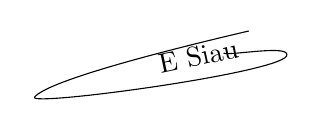
\begin{tikzpicture}[scale=.8]
\node[rotate=12] at (.5,.2) {\unsure{E Siau}};
\draw (1.3,.6) .. controls (-.2,.25) and (-1.9,-.2) .. (-2.1,-.45) .. controls (-2.2,-.6) and (1.7,-.08) .. (1.9,.2) .. controls (2,.4) and (1,.2) .. (.9,.25);
\end{tikzpicture}}

\uline{E. SIAU}

\scanpage{57}
% archive foliation: 56
% lines 1-2, upper right
\begin{tabular}{l}
autom. des\\
groupoïdes
\end{tabular}

\scanpage{58}
% archive foliation: 57
% lines 1--4, heading and opening
\uline{Automorphismes de groupoïdes.}

1) Soient $C$ \deleted{$\unsure{=(\operatorname{Ob},\operatorname{Fl},c)}$} un groupoïde,
$C'$ une catégorie, on s'intéresse à
\[
\operatorname{Hom}(C,C')=\operatorname{Ob}\,\uline{\operatorname{Hom}}(C,C').
\]
% lines 5--9
On a
\[
\operatorname{Hom}(C,C')\longrightarrow
\operatorname{Hom}(\underbrace{\operatorname{Ob}C}_{C_0},\underbrace{\operatorname{Ob}C'}_{C'_0}).
\]
Soit
\[ f_0:C_0\longrightarrow C'_0 \]
on cherche les $f:\unsure{C-C'|C\to C'}$ qui lui donnent naissance. On trouve :

% lines 10--16
\uline{Proposition} a) Pour qu'il existe un $f$ au dessus de $f_0$, il f. et il s.
que pour $x,y\in C_0$ appartenant à la $=$ comp. connexe de $C$
(i.e. tels que $\operatorname{Hom}_C(x,y)\ne\varnothing$) on ait
$f_0(x)\simeq f_0(y)$.

\deleted{b) \unsure{Supposons} \unsure{cette condition satisfaite}.}
% lines 17--20
b) Pour $\forall$ composante connexe $C(i)$ de $C$, soit $a_i\in C(i)_0$,
et pour $\forall$ $x\in C(i)_0$, soit
$u_x:a_i\overset{\sim}{\longrightarrow}x$. Alors
% lines 21--22, lower edge
\[
\begin{aligned}
\operatorname{Hom}_{f_0}(C,C')&\overset{\sim}{\longrightarrow}
\prod_{\deleted{\unsure{x\in}}\,C_0\setminus\{a_i\}}
\unsure{\operatorname{Isom}}(f_0(a_{i(x)}),f_0(x))\\
&\qquad\times\prod_i\operatorname{Hom}(\operatorname{Aut}(a_i),\operatorname{Aut}\unsure{(f_0(a_i)}
\end{aligned}
\]
% The final expression meets the lower and right image edges; no unseen closing signs supplied.

\scanpage{59}
% archive foliation: 58
% lines 1--2
\[
f\longmapsto\left(
\left(\underbrace{\unsure{f_0(u_x)|f(u_x)}}_{\ell_x}\right)_{x\in C_0},
\left(f_{a_i,a_i}:\underbrace{\operatorname{Aut}(a_i)\longrightarrow
\unsure{\operatorname{Aut}}(f_0(a_i))}_{\varphi_i}\right)\right).
\]
% lines 3--4
c) Pour que $f$ soit fidèle, il f. et suffit que $\forall i\in I$, $\varphi_i$ soit injectif.

% lines 5--8
Pour que $f$ soit pleinement fidèle, il f. et suffit que ;
$1^\circ)$ pour $i\ne j$, on ait
$\operatorname{Hom}(f_0(a_i),f_0(a_j))=\varnothing$

% lines 9--10
$2^\circ)$ pour $\unsure{\forall i|\forall}\ x,y\in C(i)_0$,
\[
\unsure{\operatorname{Isom}}(f_0(x),f_0(y))\overset{\sim}{\longrightarrow}
\operatorname{Hom}(f_0(x),f_0(y))
\]
% line 11
$3^\circ)$ $\forall i\in I$, $\varphi_i$ est un iso.

% lines 12--16
\deleted{\unsure{d)} Si $C$}

Pour que $\unsure{f}$ soit une équivalence,
il f. et s. qu'on ait de plus

$4^\circ)$ Tout $x'\in C'_0$ est isomorphe à un des $f_0(a_i)$

% lines 17--21
Pour que $f$ soit un isom.,
il \unsure{f.} et s. qu'on ait $1^\circ$, $2^\circ$, $3^\circ$,
et de plus

$4'^\circ)$ $f_0$ bijective.

\scanpage{60}
% archive foliation: 59
% lines 1--6, cancelled block
\deleted{
$C=(C_0,C_1)$ groupoïde connexe

$G=\operatorname{Aut}(C)$ groupe des automorphismes

$G^0$ \unsure{ss-gps} des $g\in G$ induisant l'identité sur $C_0$

\diagram{\begin{tikzcd}[column sep=large]
1\arrow[r]&G^0\arrow[r]&G\arrow[r,"{\uuline{\text{surj}}}"']&\unsure{\mathfrak{S}_{C_0}|\mathcal{S}_{C_0}}\arrow[r]&1
\end{tikzcd}}
}
% lines 7--12, cancelled bracketed paragraph
\deleted{[Pour qu'une autoéquivalence \inserted{$u$} soit un iso,
il f. et s. qu'elle soit bijective sur les objets de $C$, et induise un
iso. \deleted{\unsure{sur les}} $\operatorname{Aut}(\unsure{x|a})\longrightarrow\operatorname{Aut}(u_0x)$
pour \uline{un} $x\in C_0$ ; d'autre part, pour toute application
$C_0\overset{u_0}{\unsure{-|\longrightarrow}}C'_0$}

% line 13
\diagram{\begin{tikzcd}[column sep=large]
1\arrow[r,dash]&\operatorname{Aut}^0(C)\arrow[r,dash]&\operatorname{Aut}C\arrow[r,dash]&\unsure{\mathfrak{S}_{C}|\mathcal{S}_{C}}\arrow[r,dash]&1
\end{tikzcd}}
% lines 14--16
\deleted{$\operatorname{Aut}^0(C)\simeq$}

$\unsure{a|0}-\,\cdot$
\diagram{\begin{tikzcd}[column sep=large]
1\arrow[r]&\operatorname{Aut}^0(C,a)\arrow[r,dash]&\operatorname{Aut}^0(C)\arrow[r]&\operatorname{Aut}(\underset{\substack{\Vert\\\operatorname{Aut}_C(a)}}{\Pi_a})\arrow[r]&1
\end{tikzcd}}
\[\unsure{1}\]
% lines 17--19
\deleted{\unsure{À}} Pour déterminer
\deleted{$\operatorname{Aut}^0(C,a)=$}
\[
\operatorname{Aut}^0(C,a)=\{f\in\operatorname{Aut}(C)\mid
\operatorname{Ob}f=\operatorname{id}\ .\
(f_a:\operatorname{Aut}(a)-\operatorname{Aut}(\underset{\substack{\Vert\\ f(a)}}{a}))=\operatorname{id}\}
\]
% lines 20--22
On considère, pour $\forall$ $x\in C_0$,
\[
\unsure{T_x|T_a}=\operatorname{Isom}(a,x),\qquad\Pi_a\text{-torseur à droite}
\]
et son commutant \deleted{$\unsure{G_x=}$} $\operatorname{Aut}(x)$

\scanpage{61}
% archive foliation: 60
% lines 1--8
\uline{Corollaire} Pour que $f$ soit un iso, il f. et s. que

a) $f$ induise
\[\pi_0(f):\pi_0(C)\overset{\sim}{\longrightarrow}\pi_0(C')\]
b) $f$ induise
\[\operatorname{Ob}f=f_0:\operatorname{Ob}(C)\simeq\operatorname{Ob}(\unsure{C'|C})\]
c) $\forall i\in I$, $f_{a_i,a_i}:\operatorname{Aut}(a_i)\simeq\operatorname{Aut}(f_0(a_i))$

% line 9
\uline{NB} $f$ équivalence $\Longleftrightarrow$ a) et c) sont vrais

% lines 10--14
\uline{Corollaire} Pour qu'une application
$f_0:C_0\longrightarrow C'_0$ provienne d'un
iso $f:C\simeq C'$, il f. et s. que

a) $f_0$ \deleted{\unsure{soit}} bijective

% lines 15--18
b) $f_0$ transforme la relation d'équivalence de $C_0$ (par comp. connexes)
en celle de $C'_0$ (condition vide si $C,C'$ connexes).

% lines 19--20
c) $\forall i\in I$, $\operatorname{Aut}(f_0(a_i))$ est isom. à $\operatorname{Aut}(a_i)$.

\medskip\centerline{\rule{2cm}{0.3pt}}\medskip
% lines 21--24
\deleted{\unsure{On}} Supposons $C=C'$. Alors on trouve
\[\operatorname{Aut}(C)\longrightarrow\unsure{\mathfrak{S}_{C_0}|\mathcal{S}_{C_0}}\qquad\uline{\text{surjective}}\]
si $\operatorname{Aut}^0(C)$ est le noyau, on trouve donc

\scanpage{62}
% archive foliation: 61
% lines 1--2
On trouve
\[
\operatorname{Aut}^0(C,a)\simeq\prod_{x\in C_0\setminus\{a\}}
\deleted{\unsure{G_x}}\Pi_x
\]
\figure{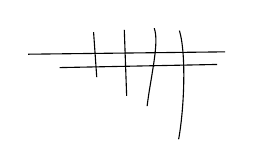
\begin{tikzpicture}[x=1cm,y=1cm]
\draw (0,0)--(2.5,.03);\draw (.4,-.17)--(2.4,-.13);
\draw (.83,.28)--(.87,-.29);\draw (1.22,.31)--(1.25,-.53);
\draw (1.6,.33)..controls(1.67,.15)and(1.55,-.31)..(1.51,-.66);
\draw (1.92,.3)..controls(2.01,0)and(1.98,-.7)..(1.91,-1.08);
\end{tikzpicture}}
% line 3
\deleted{Soit $K$ \unsure{un groupoïde}}
% lines 4--9
Soit $I$ un ensemble muni d'une structure polygonale d'ordre $n\ge2$
\deleted{\unsure{i.e.} $\unsure{\Delta_0}$}
[pour $n=2$, il faut se donner \unsure{l'ens.} des arêtes $I^*$,
\inserted{de cardinal $2$} \deleted{et}
\deleted{cardinal $2$, et}
ou ce qui revient au $=$, $\Omega(\Pi)\simeq I\wedge I^*\ \ldots$],
$\unsure{G|D}$ $(\simeq D_n)$ le \unsure{gpe|groupe} des autom. de $I$.

% lines 10--14
Soit $K=K(I)$ le graphe donné par
\[
\begin{array}{ll}
\uline{\text{Sommets}}:&\unsure{\operatorname{Ob}(\Pi)|\operatorname{Ob}(K)}=C_0=\{o,o'\}\\[4pt]
\uline{\text{arêtes}}&\unsure{I^*|I}\quad(\text{indexation }(\ell_i)_{i\in I})
\end{array}
\]
\deleted{\unsure{Relation d'incidence}}

Incidences : $C_0\times I$ (\unsure{tte} arête incidente à \unsure{tt} \unsure{sommet|sommets})
% lines 15--17, interlinear addition
\inserted{$G$ opère sur $K(I)$, et on a aussi l'\uuline{involution} $\tau$
qui est l'identité sur $I$, et échange $o,o'$, commutant à $G$.}
% lines 18--22 and left drawing
\begin{minipage}{.24\linewidth}
\figure{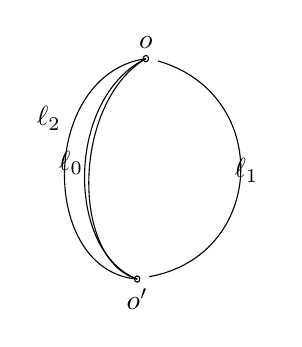
\begin{tikzpicture}[x=.85cm,y=1cm]
\coordinate (a) at (1,2.8);\coordinate (b) at (.87,0);
\draw (a)..controls(-.6,2.6)and(-.6,.1)..(b);
\draw (a)..controls(-.2,2.3)and(-.2,.35)..(b);
\draw (a)..controls(-.1,2.25)and(-.13,.25)..(b);
\draw (1.18,2.77)..controls(2.9,2.35)and(2.8,.3)..(1.05,.03);
\draw (a) circle(.04);\draw(b)circle(.04);
\node[above]at(a){$o$};\node[below]at(b){$o'$};
\node at(-.45,2.04){$\ell_2$};\node at(-.12,1.48){$\ell_0$};\node at(2.5,1.38){$\ell_1$};
\end{tikzpicture}}
\end{minipage}\hfill
\begin{minipage}{.72\linewidth}
Soit $C(I)$ le groupoïde fondamental de $K(I)$.
\deleted{le groupe} $G$ y opère par automorphismes, en opérant transitivement sur $C_0=\{o\ o'\}$.
\end{minipage}

% line 23
On va regarder le \deleted{commutant}\inserted{normalisateur de $G$} dans

\scanpage{63}
% archive foliation: 62
% lines 1--2
$G$ dans $\operatorname{Aut}(C(I))$. On a un élément canonique $\tau$
% Faint offset impressions and paper marks below the two written lines are not additional legible writing on this face.

\scanpage{64}
% archive foliation: 63
% lines 1--8, left diagram
\diagram{\begin{tikzcd}[row sep=1.8cm,column sep=.8cm]
&&E^+\arrow[dddl,"p_{20}^+"']\arrow[dddr,"p_{01}^+"]\arrow[dddr,phantom,"{\deleted{\unsure{\pi_1^+}}}",near end]
\arrow[d,dashed,"{\unsure{p_{12}^+}}"']
\arrow[ddd,"\pi_0^+",near end]
\arrow[ddl,"\pi_2^+"']\arrow[ddr,dashed,"\pi_1^+"]&&\\
&&\unsure{D_{12}}\arrow[dl,"q_{21}"]\arrow[dr,dashed,"q_{12}"']&&\\
&S_2&&S_1&\\
&D_{20}\arrow[r,"q_{02}"']\arrow[u,"q_{20}"]&S_0&D_{01}\arrow[l,"q_{01}"]\arrow[u,dashed,"q_{10}"']&\\
&&E^-\arrow[ul,"p_{20}^-"']\arrow[ur,"p_{01}^-"]
\arrow[uuu,dashed,"{\unsure{p_{12}^-}}",shift left=1.5ex]
\arrow[u,"\pi_0^-"']\arrow[uul,dashed,"\pi_2^-"']\arrow[uur,dashed,"\pi_1^-"]&&
\end{tikzcd}}
% lines 1--3, upper right formulas
\[
\left\{\begin{aligned}
\rho_0^+&=(p_{\unsure{01}}^+)^{-1}p_{01}^-(p_{20}^-)^{-1}\unsure{p_{20}^+}\\
\rho_{\unsure{1}}^+&=(p_{12}^+)^{-1}p_{12}^-(p_{01}^-)^{-1}p_{01}^+\\
\rho_2^+&=(p_{20}^+)^{-1}p_{20}^-(p_{12}^-)^{-1}p_{12}^+
\end{aligned}\right.
\qquad\rho_2^+\rho_1^+\rho_0^+=\operatorname{id}_{E^+}
\]
% lines 4--6, right quotient identities
\[
\begin{aligned}
S_0&\simeq E^+/\rho_0^+\simeq E^-/\rho_0^-\\
S_1&\simeq E^+/\rho_1^+\simeq E^-/\rho_{\unsure{1|0}}^-\\
S_2&\simeq E^+/\rho_2^+\simeq E^-/\rho_2^-
\end{aligned}
\]
% lines 7--9, right lower formulas
\[
\left\{\begin{aligned}
\rho_0^-&=(p_{01}^-)^{-1}p_{01}^+(p_{20}^+)^{-1}p_{20}^-\\
\rho_1^-&=(p_{12}^{\unsure{-}})^{-1}p_{\unsure{20}}^+(p_{01}^+)^{-1}p_{01}^-\\
\rho_2^-&=(p_{20}^-)^{-1}p_{20}^+(p_{12}^+)^{-1}p_{12}^-
\end{aligned}\right.
\]

\scanpage{65}
% archive foliation: 64
% lines 1--2, upper right title
Sous groupes finis de
$\operatorname{GP}(1)$ (cas \uline{tame})
% line 3, separate upper-left mark
\margin{\unsure{S.|5.}}

\scanpage{66}
% archive foliation: 65
% lines 1--3, upper margin and first display
\margin{En \unsure{galoisien} $d_{ij}=\deleted{\unsure{N}}d_i=N/\nu_i$}
\[
\begin{aligned}
2-2g'&=N(2-2g)\unsure{-}\underbrace{(N\nu\unsure{-|+}\nu')}_{\sum_{i,j}(d_{ij}-1)}\\
&=N(2-2g)-\sum_i\underbrace{\nu_i(N/\nu_i-1)}_{N-\nu_i=N(1-\frac{\nu_i}{N}}
\end{aligned}
\]
\deleted{$\unsure{g'}$}\qquad\deleted{$\unsure{Nd}$}
% line 4
\[
\boxed{2-2g'=N\left[(2-2g)-\sum_i\left(1-\frac1{d_i}\right)\right]}
\]
% lines 5--7
Si $g'=0$, on trouve $g=0$ et
\[
\boxed{\frac2N=2-\sum_i\left(1-\frac1{d_i}\right)>0}
\]
d'où
\[\sum_i\left(1-\frac1{d_i}\right)<2\]
% line 8
\uline{Obs} Tous les $d_i\ge2$ \deleted{\unsure{car}} ici $I$ est \uline{\unsure{tout}} l'\unsure{ens.} de ramification

% lines 9--10
1) $\operatorname{Card}I=0$\qquad $\frac2N=2$, $N=1$ : \deleted{\unsure{pour}} $G=1$

% lines 11--14
2) $\operatorname{Card}I=1$
\[
\frac2N=2-\left(1-\frac1d\right)=1+\frac1d\qquad
2=N+\frac Nd=N+\nu
\]
\margin{or $N\ge1$, $\nu\ge1$\par donc $N=1$, $\nu=1$\par $I=\varnothing$}
\uline{impossible}

% lines 15--17
3) $\operatorname{Card}I=2$
\[
\frac2N=\frac1{d_1}+\frac1{d_2}\qquad
2=\frac N{d_1}+\frac N{d_2}=\nu_1+\nu_2\qquad
\nu_1,\nu_2\ge1\qquad\nu_1=\nu_2=1
\]
\[d_1=d_2=N\qquad\uline{N\text{ quelconque}}\]

% lines 18--21
4) $\operatorname{Card}I=3$
\[
\deleted{\unsure{\frac2N=2}}\qquad
\frac1{\unsure{p|d_1}}+\frac1{\unsure{q|d_2}}+\frac1{\unsure{d_3|r}}>1
\qquad\left(\frac2N=\left(\frac1p+\frac1q+\frac1r-1\right)\right)
\]
OPS\qquad $\unsure{p\ge q\ge r}$

% lines 22--26
 a) $\unsure{r|p}=2$\qquad $\frac1p+\frac1q>\frac12$\qquad
 i.e. posant $p=\alpha+2$, $q=\beta+2$\qquad $(\alpha\ge\beta\ge0$
\margin{\deleted{$\unsure{\alpha}$}}
\[
2p+2q-pq>0\qquad
\begin{gathered}
\deleted{\unsure{2(\alpha+\beta)+8-}}\\
\underbrace{2(\alpha\unsure{+|-}2)+2(\beta+2)-(\alpha+2)(\beta\unsure{+|-}2)}_{4-\alpha\beta>0}>0
\end{gathered}
\]
\[
\alpha\beta<4\qquad
\begin{aligned}
\beta&=0,\quad\alpha\ \text{quelc.}\\
\beta&=1,\quad\alpha=1,2,3\\
&\deleted{\unsure{\beta=2,\alpha}}
\end{aligned}
\]
% lines 27--30
\[
\left\{\begin{array}{lll}
(2,2,p)&p\ge2\ \text{quelc.}&N=2p\\
(2,3,3)&&N=12\\
(2,3,4)&&N=24\\
(2,3,5)&&N=60
\end{array}\right.
\]
% line 31
b) $r\ge3$\qquad $\frac1p+\frac1q>1-\frac1r\ge\frac23$\qquad
\uline{impossible} car $\frac1p,\frac1q\le\frac13$

% lines 32--34, lower edge
5) $\operatorname{Card}I\ge4$\qquad
$\deleted{\unsure{\sum}}\quad\frac1p+\frac1q+\frac1r+\frac1s>2$\qquad
$\deleted{\unsure{\forall}}\ \unsure{p\ge q\ge r\ge s}$

Faisons d'abord $\operatorname{Card}I=4$
\[
\deleted{\frac1p+\frac1q+\frac1r>2-\frac1s=1+(1-\frac1s)\ge1+(1-\frac1p)>1}
\]

\scanpage{67}
% archive foliation: 66
% lines 1--8, letterhead
\begin{minipage}{.45\linewidth}\centering
U N I V E R S I T E\\
DES SCIENCES ET TECHNIQUES\\
DU LANGUEDOC\\
------------\\
Service de la Scolarité\\
MR / GJ\\
Diffusion : Liste A\\
N° : 4066
\end{minipage}\hfill
\begin{minipage}{.48\linewidth}
Montpellier, le 28 Juin 1978
\end{minipage}

% lines 9--10
\begin{center}
\uline{AVIS DE SOUTENANCE D'UNE THESE DE DOCTORAT DE 3ème CYCLE}

\uline{( CHIMIE ORGANIQUE PHYSIQUE )}
\end{center}

% lines 11--14
\uline{Nom et prénom du candidat} :\qquad AURELLY Michèle

\uline{Titre de la thèse} : Application de la corrélation de Hammett à l'étude de
l'énolisation des cétones en milieux basique et superbasique.

% lines 15--17
\uline{Date, heure et lieu de soutenance prévus} :
\begin{flushright}
JEUDI 13 JUILLET 1978 à 16 Heures\\
Salle de cours n° 9 - U. S. T. L.
\end{flushright}

% lines 18--21
\uline{Nom du Directeur de thèse} :
\begin{flushright}Monsieur le Professeur LAMATY.\end{flushright}

\uline{Désignation du laboratoire où la thèse est préparée} :
\begin{flushright}Laboratoire de Chimie Organique Physique.\end{flushright}

% lines 22--27
\uline{Analyse de l'ouvrage} :

Ce travail consiste à cerner de plus près
les mécanismes de l'énolisation des cétones par l'étude d'acétophénones et
de méthyl-2 phényl-1 butanones-1 substituées, dans des milieux basiques.
Les constantes \unsure{$p$|$\rho$} de Hammett ont été mesurées en fonction de la nature du milieu.

% lines 28--34
\uline{Durée approximative des recherches ayant abouti à la thèse : 3 ans.}

\uline{Composition du jury proposé} :
\begin{center}
MM. :\\
LAMATY, Président\\
SCHUE\\
WYLDE\\
MION
\end{center}

% lines 35--37, signature
\begin{flushright}
Le Secrétaire Général,

\figure{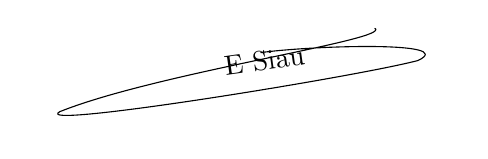
\begin{tikzpicture}[x=1cm,y=1cm]
\node[rotate=8] at(2.7,.6){\unsure{E Siau}};
\draw(4.1,1.01)..controls(4.35,.87)and(1.35,.45)..(.1,-.05)
..controls(-.3,-.28)and(3.85,.39)..(4.65,.6)
..controls(5.18,.85)and(3.3,.79)..(2.65,.7);
\end{tikzpicture}}

\uline{E. SIAU}
\end{flushright}

\scanpage{68}
% archive foliation: 67
% lines 1--7, diagonally cancelled calculation
\deleted{
$(p,q,r)$ doit être parmi les \deleted{\unsure{trois}} syst. \unsure{énumérés}

a) $p,2,2$ : $\frac1p+\frac12+\frac12>(1+(1-\frac1s)$\qquad
i.e. $\frac1p+\frac1s>1$ impossible car $\frac1p,\frac1s\le\frac12$

b) $(p,3,2)$ $(p=3,4,5\unsure{)},s\ge p)$
\deleted{$\unsure{\frac1p+\frac13+\frac12}$}
\[
\frac1{\unsure{s|p}}+\frac1p+\underbrace{\frac13+\frac12}_{5/6}>2
\qquad\frac1s+\frac1p>\frac76\quad\text{impossible car }\frac1s,\frac1p\le\frac13
\]
}
% lines 8--11, live calculation
\[
\frac1p+\frac1q>2-\underbrace{\left(\frac1r+\frac1s\right)}_{\substack{\le1\\\text{car }1/r\le1/2\\1/s\le1/2}}\ge1
\quad\text{donc}\quad\frac1p+\frac1q\ge1\quad\text{impossible car }\frac1p,\frac1q\le\frac12
\]
\uline{Impossible} !

% lines 12--14
Car si $\operatorname{Card}I\ge4$, on aura
\[
\frac1{d_1}+\frac1{d_2}+\frac1{d_3}+\frac1{d_4}
\deleted{\unsure{+\sum_{5\le i\le\nu}\frac1{d_i}}}
>\begin{array}{c}\unsure{2}+\sum_{5\le i\le\unsure{\nu}}(1-\frac1{d_i})\\\unsure{\vee}\\2\end{array}
\]
et on vient de voir que c'est impossible !

% lines 15--20, lower draft crossed in large X strokes
\deleted{
\uline{Étude du cas} \deleted{$\unsure{\operatorname{Card}I=2}$}\inserted{$(N,N)$} :
En caractéristique $0$, c'est le cas \unsure{kummérien},
\[G\simeq\mu_N(k)\simeq Z/NZ\qquad\ldots\]
\deleted{\unsure{Plus}} \unsure{gén.}, il en est ainsi si car. $p$ premier à $N$

Si $p\mid N$, on trouve une \inserted{$p$-}extension
\inserted{(de degré $p^r$, \unsure{t.t.} ramifiée et \unsure{inséparable})}
d'une $N'$-extension kummérienne $(N=p^rN',\ (p,N')=1)$.
C'est donc une
% lines 21--26, multiple revisions within the cancelled draft
\uline{extension} \deleted{est} \uline{résoluble},
\deleted{On en peut dire plus,}
\inserted{mais bien mieux : les $p$-\deleted{\unsure{extensions}}sous-groupes
\inserted{$H$} de $\operatorname{GP}(1,k)$ sont abéliens et contenus dans}
\deleted{\unsure{dans un grpe} \illegible{1}. (\unsure{car} \illegible{4})}
\margin{\unsure{conjugués} entre eux, et $H$ isom. à $(Z/pZ)^{\unsure{r|\nu}}$.}
\deleted{\unsure{abélien unipotent}}
sous-groupes \unsure{unip\textsuperscript{ts}} de dim $1$, On trouve donc
% lines 27--30
$G\subset\text{Borel}$, et par suite $G$ produit $\frac12$ direct d'un
groupe cyclique premier à la car., par un $(Z/pZ)^r$.
En fait, on voit aisément (\deleted{\unsure{encore}}
\unsure{puisqu'on est dans le cas} (cyclique premier à car., donc kummérien, qui en est exclu),
on \unsure{tombe en contradiction}.

% margin beside lines 28--32
\margin{En tous les cas, \unsure{on a une} extension abélienne
\unsure{non kummérienne|ou kummérienne}
(d'ordre premier à $p$) \unsure{par un grpe}
$\unsure{(Z/p^nZ)^\nu|(Z/pZ)^\nu}$}

% lines 31--37
\uline{Étude du cas} $(\unsure{N},2,2)$, $(\unsure{[G]}=2N)$.
En car. $\ne2$, \uline{\unsure{l'indice}}\inserted{\unsure{d'ordre} \unsure{vt}}
de ramification $2$ \unsure{en|est} ramification modérée, et faisant une
\deleted{\unsure{d'ordre} \illegible{1}}
extension kummérienne de degré $2$, on \deleted{\unsure{en}} trouve
un $X'/Y'$ qui n'a plus que $2$ pts de ramification \deleted{dans} $Y'$
\diagram{\begin{tikzcd}
X\arrow[d]&X'\arrow[l]\arrow[d,dash]\\
Y&Y'\arrow[l]
\end{tikzcd}}
donc $X'/Y'$ est justiciable de l'étude précédente
mais \unsure{pb} \deleted{\unsure{faut vérifier}} \deleted{\unsure{que si}}
$X'$ de genre $0$ (facile)
}

\scanpage{69}
% archive foliation: 68
% lines 1--10
\begin{center}U N I V E R S I T E\\DES SCIENCES ET TECHNIQUES\\DU LANGUEDOC\\------------\\Service de la Scolarité\\MR/GJ\\Diffusion : Liste A\\N°:4000\end{center}
\begin{flushright}Montpellier, le 26 Juin 1978\end{flushright}
\begin{center}\uline{AVIS DE SOUTENANCE D'UNE THESE DE DOCTORAT D'UNIVERSITE}\end{center}
% lines 11--20
\uline{Nom et prénom du candidat} : PAYEN Jean-Luc

\uline{Titre de la thèse} : Contribution à l'étude de la protection des surfaces métalliques par les composés oxyfluorés du phosphore V.

\uline{Date, heure et lieu de soutenance prévus} :
\begin{quote}13 JUILLET 1978 à 11 Heures\\Ecole Nationale Supérieure de Chimie.\end{quote}
\uline{Nom du Directeur de thèse} :
\begin{quote}Monsieur le Professeur L. COT.\end{quote}
\uline{Désignation du laboratoire où la thèse est préparée} :
Laboratoire de Chimie minérale appliquée - Chimie des Matériaux, E. N. S. C. M.
% lines 21--28
\uline{Analyse de l'ouvrage} :

Les sels de l'anion $\mathrm{PO3F}^{2-}$ peuvent être utilisés lors de l'opération de post-traitement après phosphatation en substitution des sels de chrome VI hautement toxiques.

Une étude de la nature de la surface crée par phosphatation et passivation par K2PO3F a été entreprise par différentes techniques : ESCA,Microscopies électronique , et ionique. Elle montre une réorganisation physico chimique de la couche.
% lines 29--40
\uline{Durée approximative des recherches ayant abouti à la thèse} : 2 ans

\uline{Composition du jury proposé} :
\begin{quote}MM. :\\M. MAURIN\\L. COT\\P. DESRE\\J. DURAND\\X. GRANDIN DE L'EPREVIER\\B. PARANT\\P.R PHILIP\end{quote}
\begin{flushright}Le Secrétaire Général,\end{flushright}
\figure{
\begin{tikzpicture}[x=1cm,y=1cm]
\node[rotate=13] at (2.6,.55) {\unsure{E Siau}};
\draw (3.9,.55) .. controls (3.2,.85) and (-.4,-.15) .. (0,-.25) .. controls (.45,-.48) and (4.3,.42) .. (3.9,.55);
\end{tikzpicture}}
\begin{flushright}\uline{E. SIAU}\end{flushright}

\scanpage{70}
% archive foliation: 69
% lines 1--3, upper right
Paradigme \deleted{\unsure{topologique}}\inserted{``\unsure{gruppentheoretisch}''}
des surfaces compactes
à opérateurs.

\scanpage{71}
% archive foliation: 70
% lines 1--2
Paradigme des courbes algébriques

I\quad Point de vue topologique.
% lines 3--7
On considère des surfaces topologiques (sans bord)
orientables paracompactes \inserted{$X$} -- on se donne
 aussi un ensemble $\omega$ de cardinal $2$,
et on pose
\[T=Z\wedge_{Z/2}\omega,\]
% lines 8--14
et on suppose donnée sur $X$ une $\omega$-orientation,
i.e. une \inserted{$Z/2$-}application
\deleted{\unsure{équivariante|compatible}}\inserted{de $\omega$ dans}
l'ens. des orientations de $X$, ou ce
qui revient au $=$, un isomorphisme
du faisceau des entiers tordus sur $X$
avec le faisceau constant $T_X$.
% lines 15--22
On suppose que tte composante connexe
$X_i$ de $X$ \deleted{soit}\inserted{est} \unsure{homéomorphes|homéomorphe} à un
$\widehat X_i\setminus S_i$, où $\widehat X_i$ est une surface
compacte, et $S_i$ une partie finie de
$\widehat X_i$. On sait que $(\widehat X_i,S_i)$ est déterminé
à isom. unique près par $X_i$
(comme le \unsure{décomp.} des compactifiés de Čech

\scanpage{72}
% archive foliation: 71
% lines 1--4
 de $X_i$ suivant \unsure{ses|les} points à l'infini\ldots).
Cl. que $\widehat X_i$ est automatiquement $\omega$-orienté,
donc aussi
\[\widehat X=\coprod\widehat X_i\]
% lines 5--12
De cette façon, la catégorie envisagée
(des surfaces topologiques ``spéciales''
$\omega$-\unsure{orientées|orientation}\inserted{-- aux homéomorphismes $\omega$-orientés}) devient équivalente à
celle des surfaces topologiques \inserted{$\omega$-orientées}
à comp. conn. compactes \uline{munies}
d'une partie \deleted{\unsure{fi}} $S$ discrète,
avec les isom. de couples $(\widehat X,S)$.
% lines 13--20
De $\overline{\mathrm m}$, la catégorie des couples
\deleted{$\unsure{(X,\widehat X)|(X,o)}$} $(X,o,\unsure{J|I})$ avec $(X,o)$ comme
dessus ($o$ la $\omega$-orientation) et
$\unsure{J|I}$ partie discrète de $X$, est équivalente à celle des systèmes
$(\widehat X,o,S,\unsure{J|I})$, où $(\widehat X,o)$ est une surface
$\omega$-orientée à comp. conn. compactes,

\scanpage{73}
% archive foliation: 72
% lines 1--2
et $S,J$ sont deux parties discrètes
disjointes de $\widehat X$.
% lines 3--8
On va \deleted{\unsure{à}} passer aux catégories
isotopiques correspondantes, et
en donner des interprétations
en termes de théorie des groupes.
Bien entendu, pour cette description,
on est ramené au cas connexe.
% lines 9--16
On peut \deleted{aussi} noter tt de suite
que pour ce pb, on est ramené
au cas où $J=\varnothing$ [en \deleted{\unsure{remplaçant}}\inserted{\unsure{décrivant}}
dans le cas général comme celui
de la donnée d'un $(\widehat X,I)$
\uline{plus} la donnée d'une partie $J$
de $I$].
% lines 17--20
Mais on \unsure{gardera|garde} le
pb sous \inserted{la} forme générale, en
gardant également la dissymétrie
dans le rôle des $S,J$ -- mais

\scanpage{74}
% archive foliation: 73
% lines 1--3
on devra expliciter dans le paradigme
le passage d'une description à
l'autre.
% lines 4--9
\deleted{La description}

1) Cas $J=\varnothing$\deleted{\inserted{$S\ne\varnothing$}}.
On se suppose, pour
notre description, que l'on n'est
pas dans les cas $g=0$, $\nu=0,1$
($g$ : genre de $\widehat X$, $S=\operatorname{Card}\nu$)
% lines 10--15
On associe à $(\widehat X,\widehat o,S)$\inserted{(ou) $(X,o)$} le
groupe fondamental $\Pi=\pi_1(X)$, considéré
comme groupe extérieur, mais
muni de sa $T$-structure :
locale indexée par $S$, i.e. une
\deleted{\unsure{famille}}\inserted{application}
% lines 16--17
\deleted{$\unsure{(\varphi_s)_{s\in S}|(\rho_s)_{s\in S}}$}
\margin{\textcircled{\unsure{1°}}}
\[S\longrightarrow\deleted{\unsure{g_s}}\operatorname{Homext}(T,\Pi)\]
% interlinear insertion following the local T-structure
\inserted{Ceci permet de définir $\Pi_1\ (\simeq\pi_1(\widehat X))$ comme
\unsure{groupe quot.} de $\Pi$ par le \unsure{ss-gpe inv.} engendré par les
$T\longrightarrow\Pi$.}
\inserted{Si $\nu=0$ i.e. $S=\varnothing$, il faut de}
% left margin, continuation of the preceding insertion
\inserted{plus à donner un iso
$T\longrightarrow\bigl[(\bigwedge^2\Pi_{1\mathrm{ab}})^\vee\bigr]^{\unsure{\mathrm{prim}|\mathrm{inv}}}$
de $T$ dans les formes
\unsure{primitives|invariantes} \unsure{ss} le groupe des
\unsure{autom.} ext. de \deleted{$\unsure{\Pi}$} $\Pi_1$.}
% lines 18--21
Ceci donne \inserted{$=$} une description
$\unsure{1}$-isotopique, et $=$ $\infty$-isotopique,
sauf si $g=0$, $\nu=2$ et $g=1$, $\nu=0$,
où les composantes \unsure{neutres}

\scanpage{75}
% archive foliation: 74
% lines 1--3
 du groupe des autom. de $(X,o)$
n'est pas contractile (mais un
$K(Z,1)$ resp. un $K(Z^{\unsure{2}},1)\ldots$)
% lines 4--11
2°) $J\ne\varnothing$. On a une description
plus jolie (tjrs exception faite
des cas $g=0$, $\nu=0,1$) par le
groupoïde fondamental de $X$
en $J$, mais avec $T$-structure
\unsure{à la carte} sur le groupe extérieur
$\Pi$ associé -- et si $\nu=0$, à la place de
cette structure, il faut se donner
% line 12
\[T\hookrightarrow(\bigwedge^2\Pi_{1\mathrm{ab}})^\vee\]
% lines 13--15
comme dans 1°\ldots. Ici on trouve
une description $\infty$-isotopique, même
dans les cas $g=0$, $\nu=2$, ou $g=1$, $\nu=0$
\margin{vérifier}

\scanpage{76}
% archive foliation: 75
% lines 1--2, upper right
groupes \unsure{prolibres|problèmes}
spéciaux

\scanpage{77}
% archive foliation: 76
% upper-left diagram
\diagram{\begin{tikzcd}[column sep=small]
&R\arrow[dl,"p"']\arrow[d,bend right=16,"q'"']\arrow[d,bend left=16,"q''"]\arrow[dr,"r"]&\\
S&A&F
\end{tikzcd}}
% upper-centre diagram
\diagram{\begin{tikzcd}[column sep=large]
&R^{\unsure{o|0}}=R\arrow[dl,"p^{\unsure{o|0}}=p"']\arrow[d,bend right=16,"q'^{\unsure{o|0}}=q''"']\arrow[d,bend left=16,"{q''^{\unsure{o|0}}=\deleted{\unsure{q'}}\inserted{q'\circ\sigma_2}}"]\arrow[dr,"{\unsure{q^{o}|r^{o}}=q\circ\sigma_2}"]&\\
S&A&F
\end{tikzcd}}
% upper-middle triangle drawing
\figure{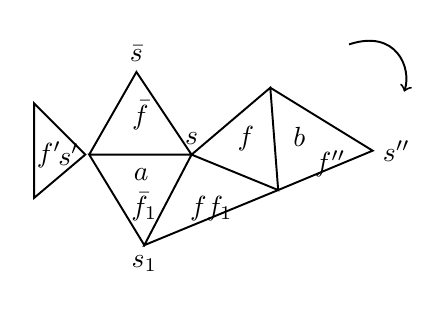
\begin{tikzpicture}[x=1cm,y=1cm,line width=.7pt]
\coordinate (s) at (2,1);\coordinate (sp) at (.7,1);\coordinate (sb) at (1.3,2.05);\coordinate (sone) at (1.4,-.15);\coordinate (r) at (3.1,.55);\coordinate (t) at (3,1.85);\coordinate (spp) at (4.3,1.05);
\draw (0,.45)--(.65,1)--(0,1.65)--cycle;
\draw (sp)--(sb)--(s)--(sp)--(sone)--(s)--(t)--(r)--(s)--(sone)--(r)--(spp)--(t);
\node at (.19,1) {$f'$};\node[left] at (sp) {$s'$};\node[above] at (sb) {$\bar s$};\node[above] at (s) {$s$};\node[below] at (sone) {$s_1$};\node[right] at (spp) {$s''$};
\node at (1.35,1.5) {$\bar f$};\node at (1.36,.75) {$a$};\node at (1.4,.34) {$\unsure{\bar f_1}$};\node at (2.69,1.2) {$f$};\node at (3.37,1.23) {$b$};\node at (3.76,.88) {$f''$};\node at (2.25,.32) {$\deleted{\unsure{f}}f_1$};
\draw[->] (4,2.4) .. controls (4.6,2.6) and (4.8,2.1) .. (4.7,1.8);
\end{tikzpicture}}
% middle-left formulae
\[\begin{aligned}
p(s,f)&=s&\sigma_0(s,f)&=(s',f')\\
r(s,f)&=f&\sigma_2(s,f)&=(s'',f'')\\
q'(s,f)&=a\\
q''(s,f)&=b
\end{aligned}\]
\[\sigma_0\sigma_2(s,f)=\sigma_2\sigma_0(s,f)=(s'',f'')\]
% upper-right display, right edge unclosed in the scan
\[E=(R,q')\times_A(R,q'')=
\left\{\overbrace{((s,f),(\bar s,\bar f))}^{\text{\unsure{rempl.}}\ (s,a,\bar f)}\mid q'(s,f)=q''(\bar s,\bar f)\right.\]
\margin{$\unsure{''}$}
% small diagram below E
\diagram{\begin{tikzcd}[column sep=small]
&E\arrow[dl,"\pi_{01}"']\arrow[d,"\pi_{02}"]\arrow[dr,"\pi_{12}"]&\\
R&R&R
\end{tikzcd}}
% middle-right displays
\[\begin{aligned}
\pi_{01}^{+}(s,f,\bar s,\bar f)&=(s,f)\\
\pi_{12}^{+}(s,f,\bar s,\bar f)&=(\bar s,\bar f)\\
\pi_{02}^{+}(s,f,\bar s,\bar f)&=(s,\bar f)
\end{aligned}\]
\[E^+=\left\{(s,f,\bar s,\bar f\unsure{]|)}\in E\mid(s,a,\bar f)\ \text{\unsure{direct}}\right.\]
\inserted{$a=q'(s,f)=q''(\bar s,\bar f)$}
% three formulae above fold
\[\left\{\begin{aligned}
\sigma_0(s,f,\bar s,\bar f)&=(s,\unsure{f_2'|f_2},\bar s,\bar f)\\
\sigma_1(s,f,\unsure{\bar s_1|\bar s},\unsure{\bar f_2|\bar f})&=(s,f_1,\unsure{\bar s'|\bar s_1},\bar f)\\
\sigma_2(s,f,\bar s,\bar f)&=(s,f,\bar s_1,\unsure{f_1|\bar f_1})
\end{aligned}\right.\]
% bottom-left diagram
\diagram{\begin{tikzcd}[column sep=small,row sep=large]
&E^+\arrow[dl,"\pi_{01}^{+}"']\arrow[d,"\pi_{02}^{+}"]\arrow[dr,"\pi_{12}^{+}"]&\\
R&R&R\\
&E^-\arrow[ul,"\pi_{01}^{-}"]\arrow[u,"\pi_{02}^{-}"]\arrow[ur,"\pi_{12}^{-}"']&
\end{tikzcd}}
% bottom-right isolated diagram objects
\diagram{\begin{tikzcd}[row sep=huge]E^+\\E^-\end{tikzcd}}

\scanpage{78}
% archive foliation: 77
% top, unfinished formula
\[\rho_0=\]
% upper-left incidence diagram
\diagram{\begin{tikzcd}[column sep=small,row sep=small]
&&E^+\arrow[dddll]\arrow[dddrr]\arrow[d]\arrow[ddl,"\pi_2^+"']\arrow[ddr,"\pi_1^+"]\arrow[ddd,bend right=4,"\pi_0^+"]&&\\
&&\deleted{D_{12}}D_{12}\arrow[ddrr,dash]&&\\
&S_2&&S_1&\\
D_{20}\arrow[uurr,dash]\arrow[rrrr,dash]&&S_0&&D_{01}\\
&&E^-\arrow[ull,dash]\arrow[urr,dash]\arrow[uuu,bend left=5]\arrow[uul,"\pi_2^-"']\arrow[uur,"\pi_1^-"]\arrow[u,"\pi_0^-"']&&
\end{tikzcd}}
% middle-right polygon drawing
\figure{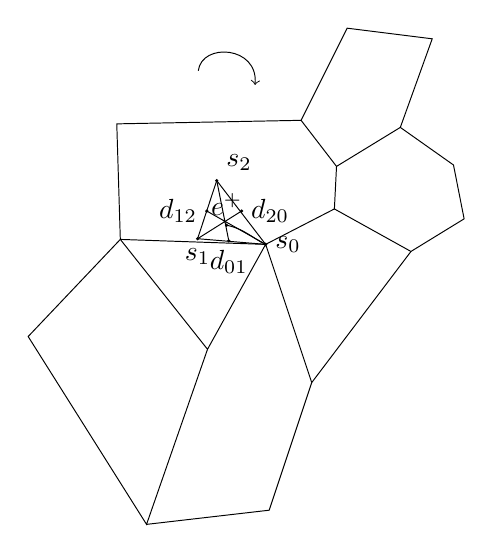
\begin{tikzpicture}[x=.009cm,y=-.009cm,line width=.35pt]
\draw (920,815)--(1180,810)--(1230,875)--(1227,935)--(1130,985)--(925,978)--cycle;
\draw (1180,810)--(1245,680)--(1365,695)--(1320,820)--(1230,875);
\draw (1320,820)--(1395,873)--(1410,949)--(1335,995)--(1227,935);
\draw (925,978)--(1048,1133)--(1130,985)--(1195,1180)--(1335,995);
\draw (925,978)--(795,1115)--(962,1380)--(1048,1133);
\draw (962,1380)--(1135,1360)--(1195,1180);
\draw[->] (1035,740) .. controls (1040,700) and (1120,705) .. (1115,760);
\coordinate (a) at (1034,977);\coordinate (b) at (1130,985);\coordinate (c) at (1061,895);\coordinate (d) at (1047,938);\coordinate (e) at (1096,938);\coordinate (f) at (1078,980);\coordinate (g) at (1075,958);
\draw (a)--(b)--(c)--cycle;\draw (c)--(f) (a)--(e) (d)--(b);
\draw (g) .. controls (1100,963) and (1114,978) .. (b);
\foreach \p in {a,b,c,d,e,f,g}{\fill (\p) circle[radius=2.5];}
\node[below] at (a) {$s_1$};\node[right] at (b) {$s_0$};\node[above right] at (c) {$s_2$};\node[left] at (d) {$d_{12}$};\node[right] at (e) {$d_{20}$};\node[below] at (f) {$d_{01}$};\node[above] at (g) {$e^+$};
\end{tikzpicture}}
% lower-left sphere drawing
\figure{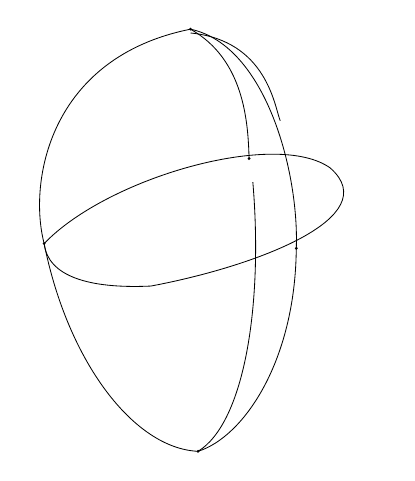
\begin{tikzpicture}[x=.012cm,y=-.012cm,line width=.3pt]
\draw (350,1238) .. controls (200,1268) and (178,1400) .. (195,1465) .. controls (220,1590) and (290,1682) .. (358,1685);
\draw (350,1238) .. controls (430,1255) and (465,1390) .. (462,1470) .. controls (461,1590) and (406,1670) .. (358,1685);
\draw (350,1238) .. controls (407,1270) and (411,1337) .. (412,1375);
\draw (416,1400) .. controls (427,1530) and (407,1655) .. (358,1685);
\draw (350,1242) .. controls (431,1250) and (439,1320) .. (445,1335);
\draw (195,1465) .. controls (262,1395) and (441,1344) .. (498,1385) .. controls (557,1437) and (420,1489) .. (308,1510) .. controls (243,1513) and (199,1500) .. (195,1465);
\foreach \p in {(350,1238),(195,1465),(412,1375),(462,1470),(358,1685)}{\fill \p circle[radius=1.6];}
\end{tikzpicture}}
% lower-left projective-line arrow
\diagram{\begin{tikzcd}\unsure{\mathbb P|P}^{1}_{\overline Q}&\unsure{\mathbb P|P}^{1}_{\overline Q}\arrow[l,"\varphi"']\end{tikzcd}}
% lower drawing, all labels and repeated pencil arcs retained
\figure{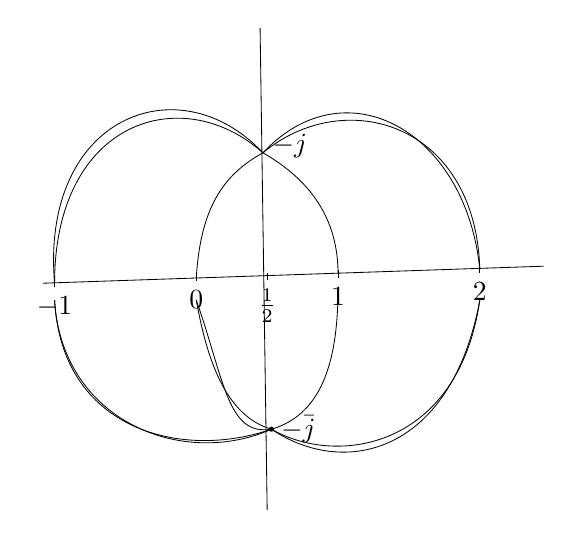
\begin{tikzpicture}[x=1.8cm,y=1.8cm,line width=.3pt]
\draw (-1.08,0)--(2.45,.12);\draw (.5,-1.6)--(.45,1.8);
\draw (-1,0) .. controls (-1,1.15) and (-.1,1.43) .. (.47,.92) .. controls (.89,.68) and (1,.36) .. (1,.065);
\draw (-1,0) .. controls (-1.1,1.18) and (-.12,1.55) .. (.47,.92);
\draw (0,.04) .. controls (.03,.52) and (.18,.76) .. (.47,.92) .. controls (1.05,1.4) and (1.97,1.13) .. (2,.1);
\draw (.47,.92) .. controls (1.05,1.54) and (1.9,1.08) .. (2,.1);
\draw (-1,-.12) .. controls (-.95,-1.04) and (-.1,-1.25) .. (.53,-1.03) .. controls (.91,-.92) and (1,-.5) .. (1,-.03);
\draw (-1,-.12) .. controls (-.95,-.97) and (-.1,-1.31) .. (.53,-1.03);
\draw (0,-.12) .. controls (.08,-.57) and (.22,-.94) .. (.53,-1.03) .. controls (1,-1.3) and (1.85,-1.16) .. (2,-.12);
\draw (0,-.12) .. controls (.2,-.69) and (.22,-1.08) .. (.53,-1.03) .. controls (1.05,-1.38) and (1.8,-1.2) .. (2,-.12);
\foreach \x/\y/\lab in {-1/0/{-1},0/.04/{0},.5/.05/{\frac12},1/.065/{1},2/.1/{2}}{\draw (\x,\y-.025)--(\x,\y+.025);\node[below] at (\x,\y-.025) {$\lab$};}
\fill (.53,-1.03) circle[radius=.018];\node[right] at (.47,.97) {$-j$};\node[right] at (.53,-1.03) {$-\bar j$};
\end{tikzpicture}}

\scanpage{80}
% archive foliation: 79
% lines 1--3
Groupe profini \uline{spécial}

\deleted{\unsure{1}} C'est un système \inserted{$\Sigma=$}
$(T,\pi,I,(\Phi_i)_{i\in I}\in(\operatorname{Homext}(T,\pi))^I$
avec
% lines 4--7
\[\Sigma\left\{\begin{array}{l}
T\ \text{groupe profini}\ \simeq\widehat Z\\
\pi\ \text{groupe profini}\\
I\ \text{ensemble fini}\\
\Phi_i\in\operatorname{Homext}(T,\pi)\qquad\text{pour }i\in I
\end{array}\right.\]
% lines 8--10
avec l'exigence que ce système est
\deleted{\unsure{équivalent}}\inserted{isomorphe}
à l'un des systèmes $\Sigma_\nu$ ($\nu\in N$, $\nu\ge1$)
suivants :
% lines 11--15
\[\Sigma_\nu\left\{\begin{array}{l}
T=\widehat Z\\
\pi=\text{groupe profini}\ \inserted{\Pi_\nu=}\widehat L_\nu,\ \text{où }L_\nu=\left\{\lambda_0,\ldots,\lambda_\nu\mid\lambda_0\lambda_1\cdots\lambda_\nu\unsure{=1}\right.\\
\qquad(\text{donc }\pi\text{ prolibre à }\nu\text{ générateurs})\\
\unsure{\Phi|I}=[0,\nu]_N\\
\Phi_i=\text{classe de l'hom }\widehat Z\xrightarrow{\varphi_i}\pi\quad\text{tel que }\varphi_i(1)=\lambda_i
\end{array}\right.\]
% lines 16--22
\uline{NB} $I$ peut être interprété comme une \uline{partie} de $\operatorname{Homext}(T,\pi)$.
Si $\Sigma\simeq\Sigma_\nu$, $\nu$ est uniquement déterminé
comme $\operatorname{card}I-1$, ou \deleted{\unsure{peut}}
\deleted{\unsure{être}} comme rang profini de $\pi_{\mathrm{ab}}$.
Pour $\nu$ fixé, la catégorie des $\Sigma$ correspondants
est équivalente à la catégorie des torseurs
sous
\[\widetilde A_\nu=\operatorname{Aut}(\Sigma_\nu)\]
% lines 23--25
On a des homomorphismes
\[\begin{aligned}
\widetilde A_\nu&\longrightarrow\unsure{\mathfrak S_{\nu+1}|\mathcal S_{\nu+1}}\ (=\operatorname{Aut}(I_\nu))\\
\widetilde A_\nu&\xrightarrow{\chi}\operatorname{Aut}\widehat Z\simeq\widehat Z^*
\end{aligned}\]

\scanpage{81}
% archive foliation: 80
% lines 1--6
donnant naissance à
\[\widetilde A_\nu\longrightarrow\unsure{\mathfrak S_{\nu+1}|\mathcal S_{\nu+1}}\times\widehat Z^*\]
qui est \uline{surjectif}. Le noyau de
$\widetilde A_\nu\to\unsure{\mathfrak S_{\nu+1}|\mathcal S_{\nu+1}}$
est noté $A_\nu$, celui de
$\widetilde A_\nu\to\unsure{\mathfrak S_{\nu+1}|\mathcal S_{\nu+1}}\times\widehat Z^*$
est noté $A_\nu^0$. D'ailleurs on a
un homomorphisme injectif
\[\pi\longrightarrow A_\nu^0\subset A_\nu\]
% lines 7--10 with interlinear addition
via automorphismes intérieurs. Le conoyau
\inserted{de $\pi\longrightarrow A_\nu^0$}
\inserted{$(\pi\to A_\nu,\pi\to\widetilde A_\nu\ \unsure{:}\ \Gamma_\nu,\widetilde\Gamma_\nu)$}
est \deleted{$\unsure{\pi}$} noté $\Gamma_\nu^0$, donc on a des
suites exactes
% lines 11--14
\[\left\{\begin{array}{l}
1\mathbin{-}\pi\mathbin{-}A_\nu^0\longrightarrow\Gamma_\nu\longrightarrow1\\
\deleted{1\mathbin{-}\pi\mathbin{-}}\\
1\mathbin{-}A_\nu\mathbin{-}\widetilde A_\nu\longrightarrow\unsure{\mathfrak S_{\nu+1}|\mathcal S_{\nu+1}}\mathbin{-}1\\
1\unsure{\Longrightarrow|\longrightarrow}A_\nu^0\longrightarrow A_\nu\mathbin{-}\widehat Z^*\mathbin{-}1
\end{array}\right.\]
% line 15
\[\overbrace{\pi\quad\Gamma_\nu^0\quad\widehat Z^*\quad\unsure{\mathfrak S_{\nu+1}|\mathcal S_{\nu+1}}}^{\unsure{\widetilde A^\nu|\widetilde A_\nu}}\qquad\text{filtration}\]
% lines 16--19
\uline{Exemples} \textcircled{1} Soit $X$ droite projective sur
$k$ alg. clos de car. $0$, $I\subset X(k)$, $\operatorname{card}I=\nu+1$
\[T=\unsure{T_\bullet(k)|T_0(k)}=\lim_{\longleftarrow\,n}\mu_n(k),\qquad\pi=\pi_1(X\setminus I,x)\]
où $x\in X(k)-I$. Il \deleted{\unsure{y}} y a par Kummer

\scanpage{82}
% archive foliation: 81
% lines 1--3
des $\Phi_i\in\operatorname{Homext}(T,\pi)$ canoniques,
$i\in I$. Le système
\deleted{$\unsure{\Sigma(X/I/k)|\Sigma(X/I/x/k)}$}\inserted{$\Sigma(X/I/x/k)$}
$=(T,I,\pi,(\Phi_i))$
satisfait aux conditions envisagées. \deleted{\unsure{Pour}}
% lines 4--7
\deleted{\unsure{Changeons}} \unsure{On}
\inserted{Au lieu de} prendre $x$, il suffit
de prendre un $\unsure{\xi|\zeta}$, foncteur fibre sur
la catégorie des rev. étales de $X\setminus I$
($\pi$ étant le groupe des autom. de $\unsure{\xi|\zeta}$\ldots)
% lines 8--11
Alors $\Sigma$ dépend fonctoriellement de
$(X/I/\unsure{\xi|\zeta}/k)$. Prenons $X/I$, $k$ fixes,
$\unsure{\xi|\zeta}$ variable, on voit que $\Sigma$ est déterminé
``mod autom. intérieurs'' i.e. \deleted{\unsure{on a}}
% lines 12--17
définit un torseur \deleted{sous}\inserted{à droite} (non pas
sous $\widetilde A_\nu$ mais sous son quotient
$\widetilde A_\nu/\pi_\nu=)\ \widetilde\Gamma_\nu$,
\deleted{le dernier torseur}\inserted{soit $P(X/I/k)$},
dont le commutant est le groupe
des ``autom. ext.'' de \deleted{$\unsure{(T,I,\pi)}$}
$\Sigma(X/I/\unsure{x|\xi}/k)\ldots$
% lines 18--20
Supposons que $X/I/\unsure{k}$ provienne
par extension de la base
\deleted{$\unsure{\operatorname{Spec}k\longrightarrow S_0}$}\inserted{$k_0\subset k$}
\deleted{d'une situation}

\scanpage{83}
% archive foliation: 82
% lines 1--3
\deleted{$X_0\unsure{/S}$} d'une situation $X_0/I_0/\deleted{k_0}k_0$
où $k_0$ est un sous-corps. [\unsure{OPS} \unsure{lors} que
$k$ \unsure{soit|est} une clôture alg. de $k_0$\ldots].
% lines 4--8
Alors $\Gamma=\operatorname{Gal}(\overleftrightarrow{k/k_0})$ opère sur
$\Sigma^{ext}$ par transport de structure, donc on a
une \deleted{la} opération aussi sur $P(X/I/k)$,
\deleted{donc} \inserted{ou encore} un hom
\[
\Gamma\longrightarrow {}^{P(X/I/k)}\widetilde\Gamma_\nu\simeq\operatorname{Aut}(\Sigma^{ext})
\]
% lines 9--11
qui par image inverse \inserted{d'extensions} donne naissance
à l'extension
\diagram{\begin{tikzcd}[column sep=small]
1\arrow[r,dash]&\pi_1(X\setminus I,\unsure{a|x})\arrow[r,dash]&\pi_1(X_0\setminus I_0,\unsure{a_0|x_0})\arrow[r]&\pi_1(k_0\unsure{/|,}k)\arrow[r,dash]&1
\end{tikzcd}}
% lines 12--13
\ldots\quad $\Gamma\xrightarrow{\chi}\operatorname{Aut}(T)\simeq\widehat{\mathbb Z}^{*}$ est l'hom de
Kummer-Tate\ldots
% lines 14--16
\textcircled{II} Plus précisément supposons $k_0=Q$, $X_0=\mathbb P^1_Q$,
\inserted{$\overline Q$ clôture alg de $Q$ dans $C$,}
\[
I=\mu_{\nu+1}(\overline Q)=\mu_{\nu+1}(C^*)\subset\overline Q=\unsure{\mathbb E^1_Q|\mathbb A^1_Q}(\overline Q)\subset\mathbb P^1_Q(\overline Q
\]
% lines 17--21
On trouve un isomorphisme canonique,
via l'exponentielle et les lacets
\[
\deleted{I\simeq[0,\unsure{\nu|2}]},
\qquad \Sigma(X/I/k)^{ext}\simeq L_\nu^{ext}
\]
donc\quad $P(X,I/k)=$ torseur trivial
